\documentclass{beamer}
\usepackage[utf8]{inputenc}
\usepackage[T1]{fontenc}
\usepackage{lmodern}  % AMS mathematical facilities for LaTeX.
\usepackage{amsthm}   % Typesetting theorems (AMS style).
\usepackage{amsfonts} % 
\usepackage{mathrsfs}
\usepackage{amsmath,fourier}
\usepackage{amssymb}
\usepackage{cancel}
\usepackage{graphicx}
\usepackage{epsfig}
\usepackage{amsmath,amsfonts,amssymb}
\usepackage{mathpazo}
\usepackage{mathtools}
\theoremstyle{remark}
\newtheorem{remark}{Remark}
\theoremstyle{plain}
\newtheorem{proposition}{Proposition}
\theoremstyle{plain}
\usetheme{Madrid} % Choose a theme (e.g., Madrid, Berlin, etc.)
\usecolortheme{default} % Choose a color theme (e.g., default, albatross, etc.)

% Customize the title page
\title[Spin-0 fields NP constants]{The cylinder at spatial infinity and asymptotic charges}
\author[Rafael Pinto]{Rafael Pinto}
\institute[CENTRA-GRIT]{Instituto Superior Técnico}
\date{October 20, 2023}
% Add a logo to the title page (optional)
\titlegraphic{
\vspace{-15mm}
\includegraphics[width=1.5cm]{centra.png}
\hspace{\fill}

\includegraphics[width=1.5cm]{grit.png}
}

\begin{document}

% Title Page
\begin{frame}
  \titlepage
  \vfill
  \begin{center}
    Advisors: \textbf{Dr. Edgar Gasper\'in} and \textbf{Dr. Alex Va\~{n}\'o - Vi\~{n}uales}
  \end{center}
\end{frame}

% Section 1: Introduction
\section{Newman-Penrose constants}
\begin{frame}{Introduction}
  \begin{columns}
    \begin{column}{0.5\textwidth}
      \begin{itemize}
      \item NP constants conserved at $\mathscr{I}$.
      \vspace{7mm}
      \item Linear theory: infinite quantities \\
      Non-linear theory: ten quantities.
      \vspace{5mm}
      \item Computed at cuts ${C} \approx \mathbb{S}^2$ of $\mathscr{I}$.
    \end{itemize}
  \end{column}
  \begin{column}{0.5\textwidth}
    \vspace*{-.8em} % Adjust the vertical position as needed
    \hfill
    \begin{figure}[h]
      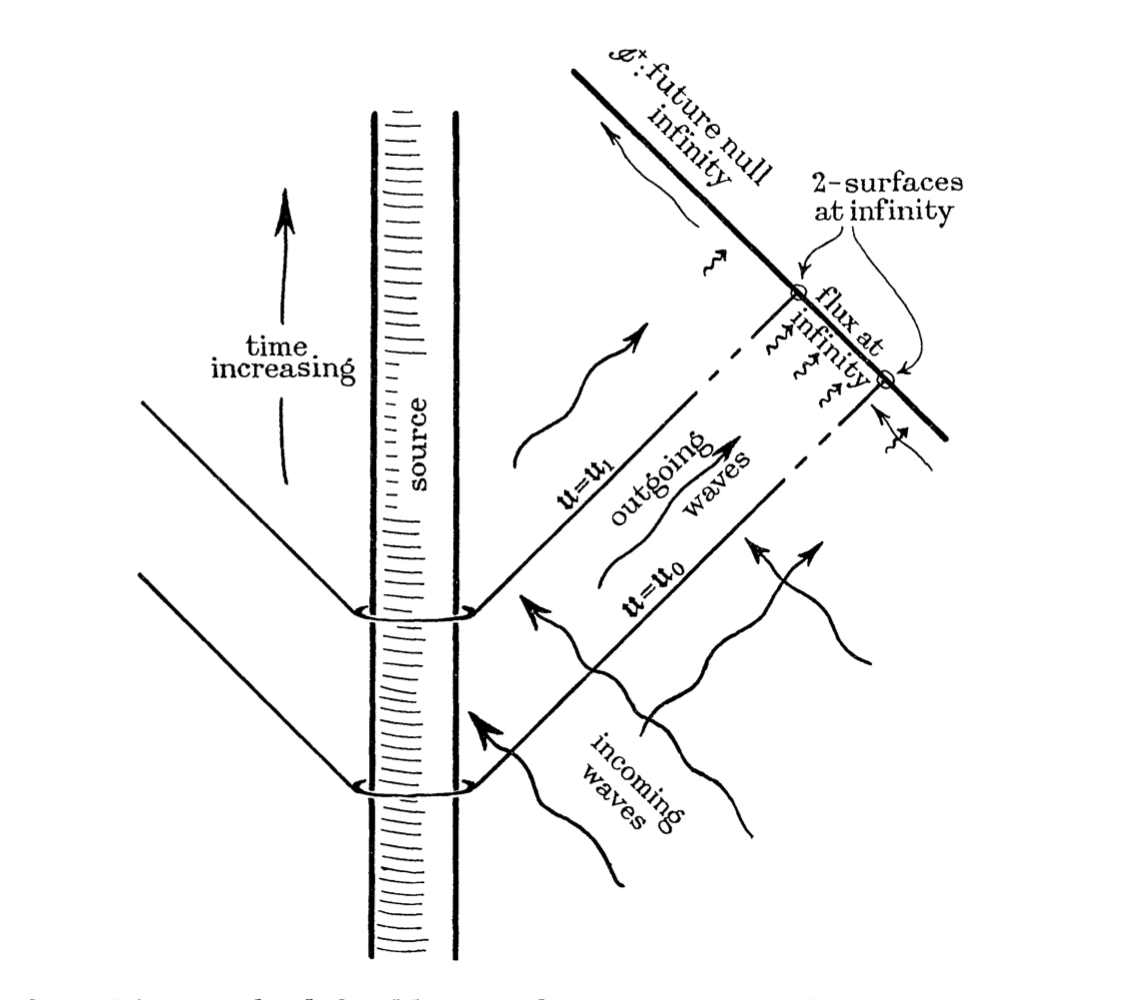
\includegraphics[width=1.2\textwidth]{penrose constants.png} 
    \end{figure}
  \end{column}
\end{columns}
\end{frame}

% Section 2: Literature Review
\section{Cylinder at $i^0$}
\begin{frame}{The $i^0$ cylinder representation in Minkowski  spacetime}
  \begin{itemize}
    \item The physical metric is given by $\tilde{\boldsymbol{\eta}}$:
    \begin{equation}
      \tilde{\boldsymbol{\eta}}=-\mathbf{d} \tilde{t} \otimes \mathbf{d} \tilde{t}+\mathbf{d} \tilde{\rho} \otimes \mathbf{d} \tilde{\rho}+\tilde{\rho}^2 \boldsymbol{\sigma}. \nonumber
    \end{equation}
    \item The conformal metric in unphysical coordinates, $\boldsymbol{\eta} = \Xi^2 \boldsymbol{\tilde{\eta}}$: 
    \begin{equation}
      \boldsymbol{\eta} = -\frac{1}{\tilde{\rho}^2 - \tilde{t}^2} (-\mathbf{d} \tilde{t} \otimes \mathbf{d} \tilde{t} + \mathbf{d} \tilde{\rho} \otimes \mathbf{d} \tilde{\rho} + \tilde{\rho}^2 \boldsymbol{\sigma}). \nonumber
    \end{equation}
    \item Introduce coordinates $(\tau, \rho, \vartheta^A)$ with $t = \rho \tau$.
    \item Consider the conformal metric $\boldsymbol{g} = \rho^{-2} \boldsymbol{\eta}$.
    \item Unphysical metric $\boldsymbol{g}$ in $F$-coordinates:
    \begin{align}
      & \boldsymbol{g} = -\mathbf{d} \tau \otimes \mathbf{d} \tau + \frac{1 - \tau^2}{\rho^2} \mathbf{d} \rho \otimes \mathbf{d} \rho - \frac{\tau}{\rho} \left(\mathbf{d} \rho \otimes \mathbf{d} \tau + \mathbf{d} \rho \otimes \mathbf{d} \tau\right) + \boldsymbol{\sigma}. \nonumber
    \end{align}
  \end{itemize}
\end{frame}

\begin{frame}
  \frametitle{Conformal Factor and Lorentz Transformation}
  \begin{columns}
    \begin{column}{0.5\textwidth}
      \begin{itemize}
        \item The conformal factor $\Theta$:
        \begin{align}
          \Theta := \rho (1-\tau^2) = \frac{1}{\tilde{\rho}}. \nonumber
        \end{align}
        \vspace{5mm}
        \item The boost parameter $\kappa$:
        \begin{align}
          \kappa := \frac{1+\tau}{1-\tau} = -\frac{\tilde{v}}{\tilde{u}}. \nonumber
        \end{align}
      \end{itemize}
    \end{column}
    \begin{column}{0.5\textwidth}
      \vspace*{-.8em} % Adjust the vertical position as needed
      \hfill
      \begin{figure}[h]
        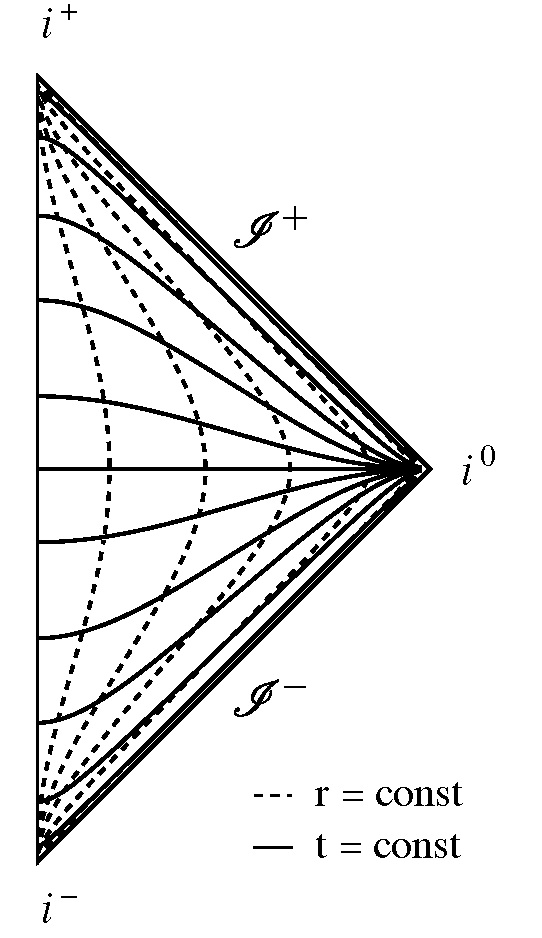
\includegraphics[width=0.65\textwidth]{Penrose diagram.pdf} % Make sure your file name matches the actual file.
        \caption{Minkowski spacetime.}
      \end{figure}
    \end{column}
  \end{columns}
\end{frame}

\begin{frame}
  \frametitle{$i^0$ Cylinder and Null Frames}
  \begin{columns}
    \begin{column}{0.5\textwidth}
      \begin{itemize}
        \item Identify $\mathscr{I}^{+}$ and $\mathscr{I}^{-}$:
        \begin{align*}
          \mathscr{I}^{+} & \equiv \{ p \in \mathcal{M} \; \rvert\; \tau(p) =1\}, \\
          \mathscr{I}^{-} & \equiv \{ p \in \mathcal{M} \; \rvert \;\tau(p) =-1\}.
        \end{align*}
        \vspace{0.4cm}
        \item The $i^0$-cylinder represents spatial infinity:
        \begin{align}
          & \mathcal{I} \equiv \{ p \in \mathcal{M} \; \rvert \;\; |\tau(p)| \leq 1, \;\rho(p)=0\}, \nonumber \\  
          & \mathcal{I}^{0} \equiv \{ p \in \mathcal{M}\; \rvert \;\tau(p)=0, \; \rho(p)=0\}. \nonumber 
        \end{align}
      \end{itemize}
    \end{column}
    \begin{column}{0.5\textwidth}
      \vspace*{-0.5em} % Adjust the vertical position as needed
      \hfill
      \begin{figure}[h]
        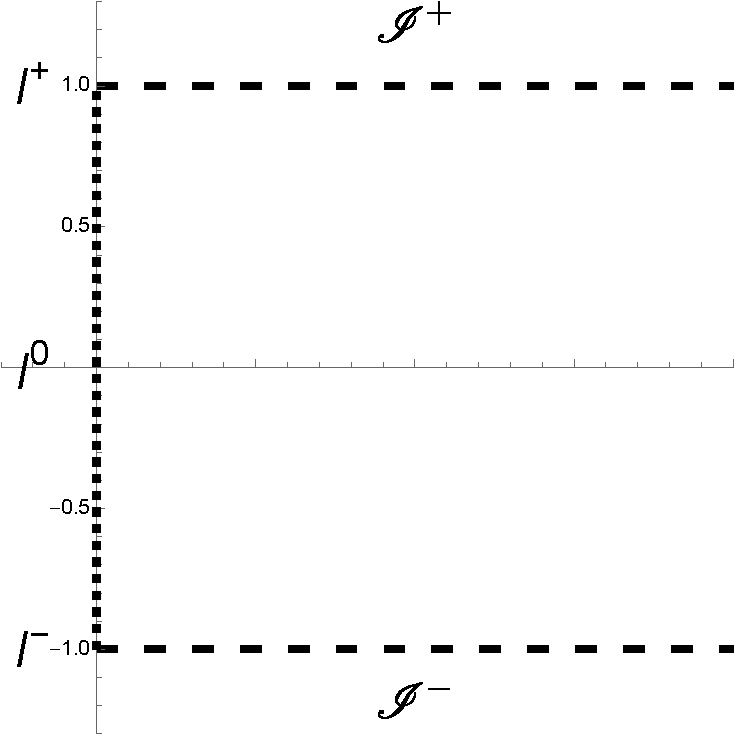
\includegraphics[width=0.9\textwidth]{friedrich cylinder.pdf} % Make sure your file name matches the actual file.
        \caption{Friedrich Cylinder.}
      \end{figure}
    \end{column}
  \end{columns}
\end{frame}

\begin{frame}
  \frametitle{$F$-Frame and Null Frames}
  \begin{itemize}
    \item Introduce the $F$-frame:
    \begin{align}
      & \boldsymbol{e}=(1+\tau) \boldsymbol{\partial}_\tau-\rho \boldsymbol{\partial}_\rho, \quad \underline{\boldsymbol{e}}=(1-\tau) \boldsymbol{\partial}_\tau+\rho \boldsymbol{\partial}_\rho, \quad \boldsymbol{e}_{\boldsymbol{A}} \quad \text { with } \nonumber \\ 
      & \boldsymbol{A}=\{\uparrow, \downarrow\}. \nonumber 
    \end{align}
    \item The NP-frame hinged at $\mathscr{I}^{\pm}$:
    \begin{align*}
      \text{NP hinged at} \; \mathscr{I}^{+}: & \quad \boldsymbol{e}^{+}, \underline{\boldsymbol{e}}^{+}, \boldsymbol{e}_{\boldsymbol{A}}^{+}, \\
      \text{NP hinged at} \; \mathscr{I}^{-}: & \quad \boldsymbol{e}^{-}, \underline{\boldsymbol{e}}^{-}, \boldsymbol{e}_{\boldsymbol{A}}^{-}.
    \end{align*}
    \item NP and physical frames:
    \begin{align*}
      \text{\emph{NP hinged at} $\mathscr{I}^{+}$}:& \quad\boldsymbol{e}^{+} = \Theta^{-2} L, \quad \underline{\boldsymbol{e}}^{+}= \underline{L},\quad \boldsymbol{e}_{\boldsymbol{A}}^{+}= \boldsymbol{e}_{\boldsymbol{A}}= \Theta^{-1}\tilde{\boldsymbol{e}}_{\boldsymbol{A}}\\ \text{\emph{NP hinged at} $\mathscr{I}^{-}$}:& \quad\boldsymbol{e}^{-} =
       L,\quad \underline{\boldsymbol{e}}^{-}=  \Theta^{-2} \underline{L},\quad \boldsymbol{e}_{\boldsymbol{A}}^{-}= \boldsymbol{e}_{\boldsymbol{A}} = \Theta^{-1}\tilde{\boldsymbol{e}}_{\boldsymbol{A}}.
    \end{align*}
  \end{itemize}
\end{frame}

% Section 3: Methodology
\section{Spin-0 fields close to $i^0$ and $\mathscr{I}$}
\begin{frame}
  \begin{itemize}
    \item The transformation of the D'Alembertian operator is,
    \begin{equation}\label{eq:waveConfTr}
      \Box \phi-\frac{1}{6} \phi R=\Omega^{-3}\left(\tilde{\Box} \tilde{\phi}-\frac{1}{6} \tilde{\phi} \tilde{R}\right). \nonumber 
    \end{equation}
    \item Using $F$-coordinates, the wave equation is represented by
    \begin{equation}\label{eq:UnphysicalWaveExplicit}
      \left(\tau^2-1\right) \partial_\tau^2 \phi-2 \rho \tau \partial_\tau \partial_\rho \phi+\rho^2 \partial_\rho^2 \phi+2 \tau \partial_\tau \phi+\Delta_{\mathbb{S}^2} \phi=0.
    \end{equation}
    \item We consider the Ansatz
    \begin{equation}\label{eq:ansatz}
      \phi = \sum_{p = 0}^{\infty}\sum_{\ell = 0}^{p}\sum_{m = -\ell}^{m = \ell}\frac{1}{p!}a_{p;\ell,m}(\tau)\rho^{p}Y_{\ell m}.
    \end{equation}
    \item Substituting \eqref{eq:ansatz} in \eqref{eq:UnphysicalWaveExplicit} simplifies to:
    \begin{equation}\label{eq:ODE_wave_JacobiPoly}
      (1-\tau^2)\ddot{a}_{p;\ell,m} + 2\tau(p-1)\dot{a}_{p,\ell,m}+(\ell+p)(\ell-p+1){a}_{p;\ell,m}=0.
    \end{equation}
  \end{itemize}
\end{frame}

\begin{frame}
  \begin{lemma}\label{Lemma:Sol_Jacobi_and_Logs} The solution to equation \eqref{eq:ODE_wave_JacobiPoly} is given
      by:
      \begin{enumerate}
      \item For $p\geq 1$ and $0\leq \ell \leq p-1$
       \begin{equation}\label{eq:Sol_jac_poly}
        a(\tau)_{p;\ell,m} =A_{p,\ell,m}\bigg(\frac{1-\tau}{2}\bigg)^{p}P_{\ell}^{(p,-p)}(\tau) + B_{p,\ell,m}\bigg(\frac{1+\tau}{2}\bigg)^{p}P_{\ell}^{(-p,p)}(\tau) \nonumber 
       \end{equation}
      
      \item For $p\geq 0$ and $\ell=p$:
         \begin{align}\label{eq:Sol_highestharmonic}
          {a}_{p;p,m}(\tau) =\bigg(\frac{1-\tau}{2}\bigg)^{p}\bigg(\frac{1+\tau}{2}\bigg)^{p}\Bigg(C_{p,p,m}+D_{p,p,m}\int_{0}^{\tau} \frac{ds}{(1-s^2)^{p+1}}\Bigg)
         \end{align}
      \end{enumerate}
  \end{lemma}
\end{frame}

\begin{frame}
  \begin{itemize}
    \item $p = 0$ and $p = 1$ cases:
    \begin{align}
      {a}_{0;0,0}(\tau) & = C_{000} + \tfrac{1}{2} D_{000} (\log(1 + \tau)- \log(1 - \tau )) \nonumber \\ 
      {a}_{1;1,m}(\tau) & = \tfrac{1}{4} (1 - \tau )(1 + \tau ) (C_{11m} + \tfrac{1}{4} D_{11m}( \log(1 + \tau ) - \nonumber \\
      & -\log(1 - \tau ) + 2\tau(1-\tau^2))). \nonumber 
    \end{align}
    \item Log terms violate peeling.
    \vspace{5mm}
    \begin{remark}\label{Remark:logfreeRemark}(Regularity condition).
      The solutions for $a(\tau)$ are polynomic in $\tau$: $D_{p,p,m} = 0$. Otherwise we need to impose the regularity condition.
    \end{remark}
  \end{itemize}
\end{frame}

\begin{frame}
  \begin{itemize}
    \item Expanding $\tilde{\phi}$:
    \begin{align}\label{eq:phi_tilde}
      & \tilde{\phi}=\Theta \phi \Leftrightarrow \tilde{\phi}=\frac{C_{000}}{\tilde{\rho}}+\frac{1}{2 \tilde{\rho}} D_{000} \log \left(\frac{\tilde{\rho}+\tilde{t}}{\tilde{\rho}-\tilde{t}}\right) Y_{00} + \frac{1}{16{\tilde{\rho}^2}} \nonumber \\
      & \left[D_{11-1}\log \left(\frac{\tilde{\rho}+\tilde{t}}{\tilde{\rho}-\tilde{t}}\right) Y_{1-1}+D_{110} \log\left(\frac{\tilde{\rho}+\tilde{t}}{\tilde{\rho}-\tilde{t}}\right) Y_{10}+\right] \nonumber \\
      & +\left[D_{111} \log\left(\frac{\tilde{\rho}+\tilde{t}}{\tilde{\rho}-\tilde{t}}\right)Y_{11}\right] + \nonumber \\
      & + \frac{1}{2 \tilde{\rho}^2}\left(A_{100}+B_{100}\right) Y_{00}+\frac{1}{4 \tilde{\rho}^2}\left(C_{11-1} Y_{1-1}+C_{110} Y_{10}+C_{111} Y_{11}\right). \nonumber 
    \end{align}
    \item In the spin-0 case, the peeling property is violated.
  \end{itemize}
\end{frame}
% Section 4: Results
\section{The NP-constants for the spin-0 fields close to $i^0$ \& $\mathscr{I}$}
\begin{frame}{The NP-constants for the spin-0 fields close to $i^0$ \& $\mathscr{I}$}
  \begin{itemize}
    \item Conservation laws:
    \begin{align*}
      {\underline{{L}}}({\tilde{\rho}}^{-2\ell}L(e^{+})^{\ell+1}\phi_{\ell m})=0, \qquad L({\tilde{\rho}}^{-2\ell}\underline{L}(e^{-})^{\ell+1}\phi_{\ell m})=0
    \end{align*}
    \item $f(\tilde{\rho})$-modified NP constants: 
    \begin{align*}
      {}^{f}\mathcal{N}^{+}_{\ell,m}:= f(\tilde{\rho})L (\boldsymbol{e}^{+})^{\ell}\phi_{\ell m} \Big|_{{C}^{+}}
    \end{align*}
    \begin{align*}
      {}^{f}\mathcal{N}^{-}_{\ell,m}:= f(\tilde{\rho})\underline{L} (\boldsymbol{\underline{e}}^{-})^{\ell}\phi_{\ell m}\Big|_{{C}^{-}}
    \end{align*}
    \item For $f(\tilde{\rho})=\tilde{\rho}^2$, classical NP-constants.
    \begin{align*}
      \mathcal{N}^{+}_{\ell,m}:= (\boldsymbol{e}^{+})^{\ell+1}\phi_{\ell m}\Big|_{{C}^{+}}
    \end{align*}
    \begin{equation}
      \mathcal{N}^{-}_{\ell,m}:= (\boldsymbol{\underline{e}}^{-})^{\ell+1}\phi_{\ell m} \Big|_{{C}^{-}} \nonumber
    \end{equation}
  \end{itemize}
\end{frame}

% Section 5: Conclusion
\section{The classical NP constants at $\mathscr{I}^{+}$}
\begin{frame}{The classical NP constants at $\mathscr{I}^{+}$}
  \begin{itemize}
    \item This analysis is facilitated by the expression,
    \begin{align*}
      \phi_{\ell m}= \sum_{p=\ell}^{\infty}\frac{1}{p!}a_{p;\ell,m}(\tau)\rho^{p}.
    \end{align*}
    \item Considering $\ell=0$, the computation of $\boldsymbol{e}^{+}(\phi_{00})$ is sufficient.
    \begin{align}
      & \boldsymbol{e}^{+}(\phi_{\ell m}) = 4 \rho^{-1}(1+\tau)^{-2}\sum_{p=0}^{\infty} \frac{1}{p!}\rho^p((1+\tau)\dot{a}_{p;\ell,m}-p a_{p;\ell,m}). \nonumber
    \end{align}
    With
    \begin{align}
      Q^{0}_{p;\ell,m}(\tau):=(1+\tau)\dot{a}_{p;\ell,m}-p a_{p;\ell,m}. \nonumber
    \end{align}
    \item With this definition in place, we can express $\boldsymbol{e}^{+}(\phi_{\ell m})$ as follows:
    \begin{align}
      \boldsymbol{e}^{+}(\phi_{\ell m}) = 4 (\Lambda_{+})^{2}\sum_{p=0}^{\infty} \frac{1}{p!}\rho^{p}Q^{0}_{p,\ell,m}(\tau). \nonumber
    \end{align}
  \end{itemize}
\end{frame}

\begin{frame}
  \begin{itemize}
    \item To compute the $\ell=0$ NP constant we evaluate at a cut ${C}^{+}$:
    \begin{align}
      \mathcal{N}^{+}_{0,0}= \lim_{\substack{\rho \to \rho_{\star} \\ \tau \to 1}}  \boldsymbol{e}^{+}(\phi_{00}) =\sum_{p=0}^{\infty} \frac{1}{p!}\rho^{p-1}_{\star}Q^{0}_{p,0,0}(\tau)|_{\mathscr{I}^{+}} = -A_{100}. \nonumber
    \end{align}
    \item To calculate the $\ell = 1$ NP constants, one has\\
    \begin{align}
      \mathcal{N}^{+}_{1,m} = \lim _{\substack{\rho \rightarrow 0 \\ \tau \rightarrow 1}}2^{-4} \frac{1}{2 !} Q^{1}_{2, 1, m}(\tau) = 3A_{21m}. \nonumber
    \end{align}
    \item The NP constants for $\mathscr{I}^{-}$ can be calculated in a similar manner, where the time reversed version of the $F$-frame is used.
  \end{itemize}
\end{frame}

\section{The $i^0$ cylinder logarithmic NP constants at $\mathscr{I}^{-}$}
\begin{frame}{The $i^0$ cylinder logarithmic NP constants at $\mathscr{I}^{-}$}
  \begin{itemize}
    \item Choice of $f(\tilde{\rho})$.
    \vspace{5mm}
    \item We will compute the $\ell=0$ and $\ell=1$ modified NP constants.
    \begin{align}
      \tilde{\rho}\underline{L} (\phi_{\ell m}) = \frac{(1+\tau)}{(1-\tau)}\sum_{p=0}^{\infty}\underline{Q}^{0}_{p;\ell,m}(\tau)\rho^p. \nonumber
    \end{align}
    Therefore, for $\ell=0$, we have:
    \begin{align}
      \mathcal{}^{\tilde{\rho}}\mathcal{N}^{-}_{0,0} = \lim_{\substack{\rho \to \rho_{\star} \\ \tau \to -1}} \; \kappa(\underline{\boldsymbol{e}^{-}})(\phi_{00}) = \sum_{p=0}^{\infty}\rho_{\star}^p\biggl[\frac{(1+\tau)}{(1-\tau)}\underline{Q}^{0}_{p;0,0}(\tau)\biggr]|_{\mathscr{I}^{-}}. \nonumber
    \end{align}
  \end{itemize}
\end{frame}

\begin{frame}
  \begin{itemize}
    \item Evaluating at the critical set $\mathcal{I}^{-}$, we obtain:
    \begin{align}
      \mathcal{}^{\tilde{\rho}}\mathcal{N}^{-}_{0,0} = \lim_{\substack{\rho \to \rho_{\star} \\ \tau \to -1}}\sum_{p=0}^{\infty}\rho_{\star}^p\biggl[\frac{(1+\tau)}{(1-\tau)}\underline{Q}^{0}_{p;0,0}(\tau)\biggr] = \frac{1}{2}D_{000}. \nonumber
    \end{align}
    \item Similarly, for $\ell=1$, the relevant quantity to evaluate is:
    \begin{align}
      \tilde{\rho} \underline{L} (\underline{\boldsymbol{e}^{-}}) \phi_{1m}= 4\kappa(\Lambda_{-})^{2}\sum_{p=1}^{\infty}\frac{1}{p!}\rho^p\underline{Q}^{1}_{p;\ell,m}(\tau). \nonumber
    \end{align}
    \item Therefore, for $\ell=1$, we have:
    \begin{align}
      \mathcal{}^{\tilde{\rho}}\mathcal{N}^{-}_{1,m} = \lim_{\substack{\rho \to \rho_{\star} \\ \tau \to -1}} \; \kappa\underline{\boldsymbol{e}}(\underline{\boldsymbol{e}^{-}})\phi_{1m} = \sum_{p=1}^{\infty}\frac{1}{p!}\rho_{\star}^{p-1}(\kappa \underline{Q}^{1}_{p;1,m}(\tau))|_{\mathscr{I}^{-}}. \nonumber
    \end{align}
    \item Evaluating at the critical set $\mathcal{I}^{-}$, we obtain:
    \begin{align}
      \mathcal{}^{\tilde{\rho}}\mathcal{N}^{-}_{1,m} = - \frac{1}{4}D_{11m}. \nonumber
    \end{align}
  \end{itemize}
\end{frame}

\section{The NP constants in terms of initial data}
\begin{frame}{The NP constants in terms of initial data}
  \begin{itemize}
    \item Classical NP Constants at $\mathscr{I}^{+}$: $\mathcal{N}^{+}_{\ell,m} = q^{+}(\ell) \;A_{\ell+1,\ell,m}$.
    \item Modified NP Constants at $\mathscr{I}^{+}$: ${}^{\tilde{\rho}}\mathcal{N}^{+}_{\ell,m} = q^{+}(\ell) \;D_{\ell,\ell,m}$.
    \item Classical NP Constants at $\mathscr{I}^{-}$: $\mathcal{N}^{-}_{\ell,m} = q^{-}(\ell) \; B_{\ell+1,\ell,m}$.
    \item Modified NP Constants at $\mathscr{I}^{-}$: ${}^{\tilde{\rho}}\mathcal{N}^{-}_{\ell,m} = q^{-}(\ell) \;D_{\ell,\ell,m}$.
    \vspace{5mm}
    \item Reminder:
    \begin{align}
      & a(\tau)_{p;\ell,m} =A_{p,\ell,m}\bigg(\frac{1-\tau}{2}\bigg)^{p}P_{\ell}^{(p,-p)}(\tau) + B_{p,\ell,m}\bigg(\frac{1+\tau}{2}\bigg)^{p}P_{\ell}^{(-p,p)}(\tau) \nonumber \\
      & {a}_{p;p,m}(\tau) =\bigg(\frac{1-\tau}{2}\bigg)^{p}\bigg(\frac{1+\tau}{2}\bigg)^{p}\Bigg(C_{p,p,m}+D_{p,p,m}\int_{0}^{\tau} \frac{ds}{(1-s^2)^{p+1}}\Bigg) \nonumber
    \end{align}
  \end{itemize}
\end{frame}
% References (optional)
\section{Conclusions}
\begin{frame}{Conclusions}
  \begin{itemize}
    \item Computed the \textcolor{red}{NP constants} for a \textcolor{red}{spin-0 field} at $\mathscr{I}$.
    \vspace{5mm}
    \item \textcolor{red}{\(D_{p;p,m} \neq 0\)}: \textcolor{red}{classical NP constants} become \textcolor{red}{undefined}.
    \vspace{5mm}
    \item \textcolor{red}{\(D_{p;p,m} = 0\)}: \textcolor{red}{classical NP constants} at \(\mathscr{I}^{\pm}\) become \textcolor{red}{defined}.
    \vspace{5mm}
    \item \textcolor{red}{Classical NP constants} $\neq$ correspondence, the \textcolor{red}{\(i^0\) cylinder NP constants} share initial data.
    \vspace{5mm}
    \item These results were published in: \textcolor{red}{J. Math. Phys. 64, 082502 (2023)} https://doi.org/10.1063/5.0158746
  \end{itemize}
\end{frame}
\end{document}
